\documentclass[11pt]{article}

\usepackage[a4paper,margin=1in]{geometry}
\usepackage{graphicx}
\usepackage{booktabs}
\usepackage{array}
\usepackage{hyperref}
\usepackage{xcolor}
\usepackage{tikz}
\usetikzlibrary{arrows.meta,positioning}

\hypersetup{
  colorlinks=true,
  linkcolor=black,
  urlcolor=blue,
  citecolor=black
}

\title{\textbf{Low-Resource Filipino Adaptation of OmniVoice for Voice Cloning and Text-to-Speech}\\
\large Research Project Proposal}
\author{Current Trends}
\date{\today}

\begin{document}
\maketitle

\begin{abstract}
Voice cloning is an emerging artificial intelligence technology that can synthesize speech in a target speaker's voice from short reference audio. Although recent multilingual text-to-speech systems support many languages, practical voice cloning workflows remain strongest in high-resource languages. This proposal investigates how much Filipino-specific fine-tuning improves the pretrained OmniVoice model using curated Filipino read speech from the UP-DSP Philippine Languages Database. The proposed study compares the base OmniVoice model with a Filipino fine-tuned checkpoint and measures the size of the change across intelligibility, naturalness, and speaker similarity metrics. The expected output is a reproducible Filipino fine-tuning workflow, generated audio samples, and an evaluation report suitable for a course-scale research project.
\end{abstract}

\section{Introduction}

Voice cloning and text-to-speech (TTS) systems have rapidly improved due to large-scale neural speech models. These systems can generate synthetic speech from text and, in zero-shot voice cloning settings, imitate a speaker's voice from a short reference recording. This capability has practical applications in education, accessibility, localization, narration, digital assistants, and language learning.

However, most high-quality voice cloning systems are built and evaluated primarily on high-resource languages such as English and Chinese. Filipino and other Philippine languages remain relatively low-resource in speech AI, which limits the quality and availability of practical Filipino voice generation tools. Instead of training a Filipino voice cloning model from scratch, this project proposes adapting an existing multilingual model: OmniVoice.

OmniVoice is a massively multilingual zero-shot TTS model that supports more than 600 languages. It includes Filipino, but the model's language table lists only about 7.71 hours of Filipino in its training mixture. This creates a research opportunity: measure how much Filipino-specific fine-tuning using a larger curated Filipino speech corpus changes the model's Filipino generation quality.

\section{Research Problem}

The research problem is that Filipino voice cloning remains underrepresented in practical open-source workflows, despite the availability of broad multilingual TTS models. OmniVoice supports Filipino, but language support alone does not guarantee optimal performance for Filipino pronunciation, rhythm, naturalness, or speaker similarity.

The proposed study asks how much a low-resource adaptation approach can improve Filipino speech generation without training a model from scratch. This is appropriate for a course-scale research project because it is experimentally measurable, technically current, and feasible using the existing OmniVoice fine-tuning pipeline.

\section{Research Question and Objectives}

\subsection{Main Research Question}

How much does Filipino-specific fine-tuning improve OmniVoice performance for Filipino TTS and voice cloning across intelligibility, naturalness, and speaker similarity metrics?

\subsection{Sub-Questions}

\begin{enumerate}
  \item How much does fine-tuning reduce Filipino character error rate or word error rate?
  \item How much does fine-tuning change objective and perceived naturalness of generated Filipino speech?
  \item How much does fine-tuning change speaker similarity in voice cloning?
\end{enumerate}

\subsection{Objectives}

\begin{enumerate}
  \item Prepare a clean Filipino speech-text dataset suitable for OmniVoice fine-tuning.
  \item Fine-tune the pretrained \texttt{k2-fsa/OmniVoice} checkpoint on Filipino read speech.
  \item Generate Filipino speech samples using both the base and fine-tuned models.
  \item Evaluate intelligibility, naturalness, and speaker similarity using objective and human evaluation methods.
  \item Produce a reproducible workflow and demo samples that can be connected to the existing voice cloning application.
\end{enumerate}

\section{Related Work}

Recent speech generation research has shifted toward large multilingual and zero-shot systems. Neural codec language models such as VALL-E showed that discrete speech tokens can be used for zero-shot TTS. Voicebox demonstrated large-scale text-guided multilingual speech generation. F5-TTS and E2 TTS explored efficient non-autoregressive TTS using flow matching, while MaskGCT used masked generative codec modeling for zero-shot TTS.

OmniVoice builds on this line of work by using a diffusion language model-style architecture for multilingual zero-shot speech generation. It directly maps text, optional language and instruction tags, and optional reference audio prompts into acoustic tokens. Unlike training a separate speaker model, OmniVoice supports zero-shot voice cloning from a short reference recording.

For Filipino data, the UP-DSP Philippine Languages Database (PLD) provides a relevant corpus for low-resource Philippine speech technology. The PLD paper reports 454:49:43 total duration across Philippine languages, including 48:56:36 of Filipino speech. This makes it suitable for an academic adaptation experiment.

\section{Selected Model: OmniVoice}

OmniVoice was selected because it is open-source, multilingual, supports voice cloning, and provides official fine-tuning scripts. The model supports more than 600 languages and includes Filipino with language ID \texttt{fil}. Figure~\ref{fig:omnivoice} shows the OmniVoice paper and Figure~\ref{fig:filipino-entry} shows the Filipino entry in the supported-language table.

\begin{figure}[htbp]
  \centering
  
\includegraphics[height=0.42\textheight,keepaspectratio]{\detokenize{../../images/omnivoice paper.png}}
  \caption{OmniVoice paper first page.}
  \label{fig:omnivoice}
\end{figure}

\begin{figure}[htbp]
  \centering
  
\includegraphics[height=0.44\textheight,keepaspectratio]{\detokenize{../../images/omnivoice filipino dataset.png}}
  \caption{OmniVoice supported-language table excerpt showing Filipino.}
  \label{fig:filipino-entry}
\end{figure}

\subsection{Architecture}

For this project, the key OmniVoice mechanism is its masked acoustic-token generation process:

\begin{enumerate}
  \item Text is encoded using a language-model tokenizer.
  \item Reference audio is converted into discrete acoustic tokens.
  \item The model receives text, language tags, and optional reference voice tokens.
  \item During training, some acoustic tokens are masked.
  \item The model learns to reconstruct the masked acoustic tokens.
  \item During inference, generated acoustic tokens are decoded into speech audio.
\end{enumerate}

Fine-tuning is expected to adapt the model's text-to-acoustic-token behavior toward Filipino speech patterns.

\section{Dataset}

\subsection{Data Source}

The primary dataset is the UP-DSP Philippine Languages Database (UP-DSP-PLD), released through Mozilla Data Collective. The dataset is distributed as WAV audio and LOG transcript files under a CC-BY-NC-4.0 license. This makes it appropriate for academic research but not for commercial deployment.

\begin{figure}[htbp]
  \centering
  
\includegraphics[width=0.95\linewidth,keepaspectratio]{\detokenize{../../images/up dsp philippine languages database.png}}
  \caption{UP-DSP PLD release page on Mozilla Data Collective.}
  \label{fig:pld-release}
\end{figure}

\subsection{Filipino Subset}

The Filipino subset is large enough for a small fine-tuning study while remaining feasible for Kaggle-based experimentation.

\begin{table}[htbp]
  \centering
  \caption{Filipino subset statistics from the PLD paper.}
  \begin{tabular}{ll}
    \toprule
    Detail & Value \\
    \midrule
    Language ID & \texttt{fil} \\
    Speakers & 135 \\
    Utterances & 52,879 \\
    Total duration & 48:56:36 \\
    Average utterance length & 3.58 seconds \\
    \bottomrule
  \end{tabular}
\end{table}

\begin{figure}[htbp]
  \centering
  
\includegraphics[height=0.43\textheight,keepaspectratio]{\detokenize{../../images/philippine languages database paper list of language.png}}
  \caption{PLD paper table showing language-level corpus statistics.}
  \label{fig:pld-table}
\end{figure}

\subsection{Read Speech Selection}

The first experiment will use Filipino read speech. Read speech is preferred because the speaker reads a prepared prompt, so the transcript is already matched to the spoken sentence. Spontaneous speech, where a speaker answers freely, may require stricter verification because the prompt or question may not equal the actual spoken transcript.

\section{Methodology}

\subsection{Data Preparation}

The data preparation process will convert Filipino WAV and LOG files into the JSONL format expected by OmniVoice:

\begin{verbatim}
{"id":"fil_000001",
 "audio_path":"/path/audio.wav",
 "text":"Magandang umaga sa inyong lahat.",
 "language_id":"fil"}
\end{verbatim}

The preparation steps are:

\begin{enumerate}
  \item Extract the Filipino subset from the PLD archive.
  \item Parse LOG files to pair each WAV file with its transcript.
  \item Keep read speech first.
  \item Filter samples to 1--10 seconds.
  \item Remove empty transcripts, invalid audio files, and placeholder transcripts.
  \item Apply light text normalization, such as trimming whitespace and removing control characters.
  \item Split the data into train, development, and test sets.
\end{enumerate}

\subsection{Fine-Tuning Pipeline}

\begin{figure}[htbp]
  \centering
  \small
  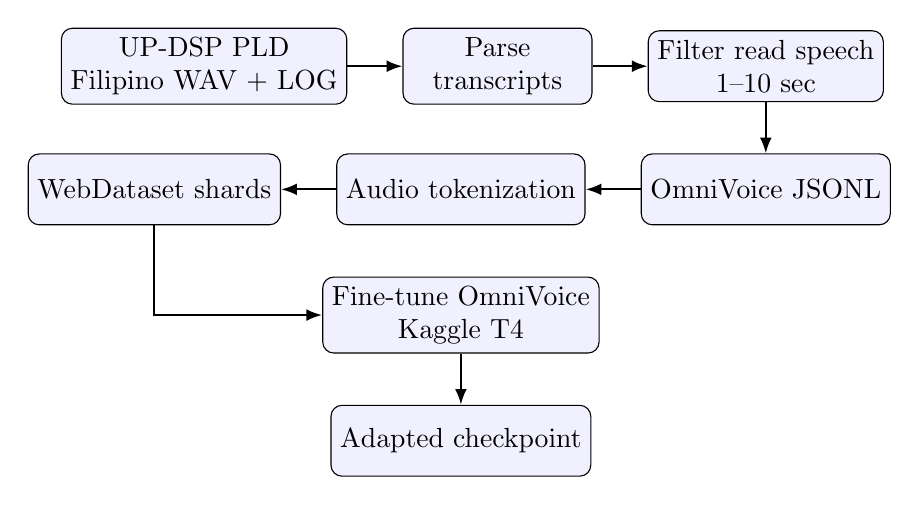
\begin{tikzpicture}[
    node distance=0.65cm and 0.7cm,
    box/.style={draw, rounded corners, align=center, minimum height=0.9cm, minimum width=2.4cm, fill=blue!6},
    arrow/.style={-{Latex[length=2mm]}, thick}
  ]
    \node[box] (a) {UP-DSP PLD\\Filipino WAV + LOG};
    \node[box, right=of a] (b) {Parse\\transcripts};
    \node[box, right=of b] (c) {Filter read speech\\1--10 sec};
    \node[box, below=of c] (d) {OmniVoice JSONL};
    \node[box, left=of d] (e) {Audio tokenization};
    \node[box, left=of e] (f) {WebDataset shards};
    \node[box, below=of e] (g) {Fine-tune OmniVoice\\Kaggle T4};
    \node[box, below=of g] (h) {Adapted checkpoint};

    \draw[arrow] (a) -- (b);
    \draw[arrow] (b) -- (c);
    \draw[arrow] (c) -- (d);
    \draw[arrow] (d) -- (e);
    \draw[arrow] (e) -- (f);
    \draw[arrow] (f) |- (g);
    \draw[arrow] (g) -- (h);
  \end{tikzpicture}
  \caption{Proposed fine-tuning pipeline.}
  \label{fig:fine-tuning-pipeline}
\end{figure}

Audio will be tokenized using the OmniVoice audio tokenizer into WebDataset shards. Fine-tuning will start from the pretrained \texttt{k2-fsa/OmniVoice} checkpoint.

\subsection{Training Environment}

The target training environment is Kaggle with 2x NVIDIA T4 GPUs. Because T4 GPUs have limited memory and do not benefit from BF16 in the same way as newer GPUs, the initial configuration will use FP16, SDPA attention, smaller token batches, and DeepSpeed ZeRO-2.

\begin{table}[htbp]
  \centering
  \caption{Initial fine-tuning configuration.}
  \begin{tabular}{ll}
    \toprule
    Setting & Planned Value \\
    \midrule
    Starting checkpoint & \texttt{k2-fsa/OmniVoice} \\
    Training data size & 5--10 hours clean Filipino read speech \\
    Precision & FP16 \\
    Attention implementation & SDPA \\
    Learning rate & 5e-6 \\
    Training steps & 1,000--2,000 \\
    Optimization & DeepSpeed ZeRO-2 \\
    \bottomrule
  \end{tabular}
\end{table}

\section{Evaluation Plan}

The study will compare two systems: the base OmniVoice checkpoint and the Filipino fine-tuned OmniVoice checkpoint. Both systems will generate speech using the same Filipino test prompts and reference voices. The goal is to quantify the size of the change for each metric, not only to state that fine-tuning helped.

\begin{figure}[htbp]
  \centering
  \small
  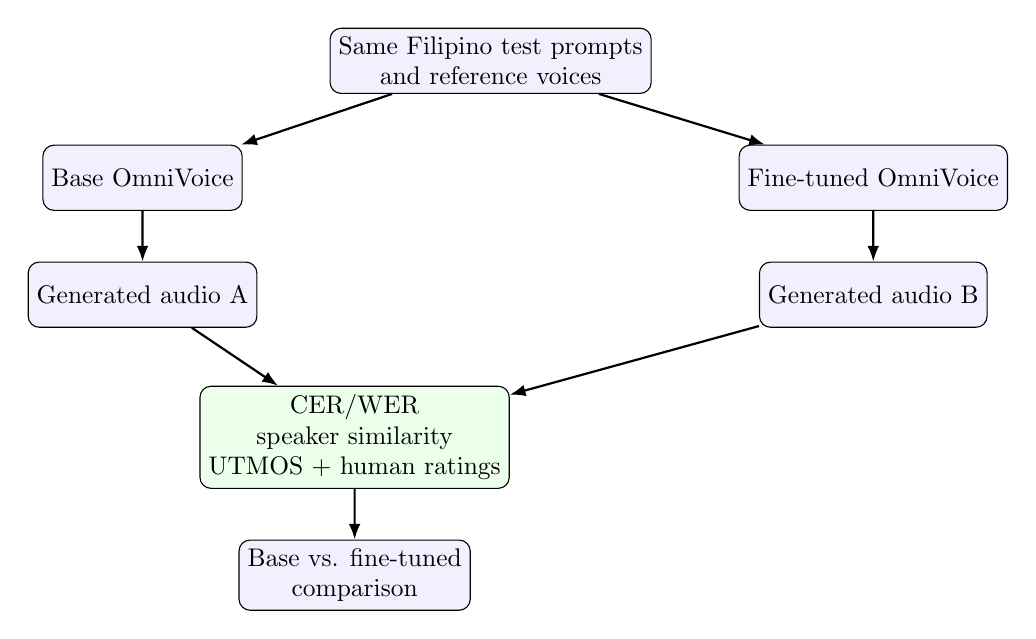
\begin{tikzpicture}[
    scale=0.92,
    transform shape,
    node distance=0.7cm and 1.2cm,
    box/.style={draw, rounded corners, align=center, minimum height=0.9cm, minimum width=2.6cm, fill=blue!6},
    metric/.style={draw, rounded corners, align=center, minimum height=0.9cm, minimum width=3.3cm, fill=green!8},
    arrow/.style={-{Latex[length=2mm]}, thick}
  ]
    \node[box] (t) {Same Filipino test prompts\\and reference voices};
    \node[box, below left=of t] (b) {Base OmniVoice};
    \node[box, below right=of t] (f) {Fine-tuned OmniVoice};
    \node[box, below=of b] (bo) {Generated audio A};
    \node[box, below=of f] (fo) {Generated audio B};
    \node[metric, below right=0.8cm and -0.8cm of bo] (m) {CER/WER\\speaker similarity\\UTMOS + human ratings};
    \node[box, below=of m] (r) {Base vs. fine-tuned\\comparison};

    \draw[arrow] (t) -- (b);
    \draw[arrow] (t) -- (f);
    \draw[arrow] (b) -- (bo);
    \draw[arrow] (f) -- (fo);
    \draw[arrow] (bo) -- (m);
    \draw[arrow] (fo) -- (m);
    \draw[arrow] (m) -- (r);
  \end{tikzpicture}
  \caption{Evaluation design.}
  \label{fig:evaluation-design}
\end{figure}

\subsection{Metrics}

\begin{itemize}
  \item \textbf{CER/WER for intelligibility:} generated audio will be transcribed by an automatic speech recognition (ASR) model and compared against the original target text. Character error rate (CER) counts character-level insertions, deletions, and substitutions; word error rate (WER) does the same at the word level. Lower values mean that the generated speech is easier for an ASR system to recognize as the intended sentence. For Filipino, CER may be useful because it is less sensitive to tokenization and word-boundary differences.
  \item \textbf{Speaker similarity for voice cloning:} reference audio and generated audio will be converted into speaker embeddings, then compared using cosine similarity. This follows the same idea as OmniVoice's SIM-o evaluation, which uses a WavLM-based ECAPA-TDNN speaker model. Higher similarity means the generated speech is closer to the reference speaker's voice.
  \item \textbf{UTMOS for objective naturalness:} if feasible, UTMOS will be used as an automatic prediction of speech naturalness. It estimates how natural or human-like a generated waveform sounds. Higher scores indicate more natural audio.
  \item \textbf{Human evaluation for listener judgment:} Filipino listeners will rate pronunciation correctness, naturalness, intelligibility, speaker similarity, and overall preference. This is important because ASR-based metrics may miss Filipino pronunciation issues, prosody, accent, or unnatural rhythm.
\end{itemize}

These metrics are aligned with the OmniVoice paper. OmniVoice evaluates intelligibility using WER or CER depending on the benchmark language, speaker similarity using SIM-o with WavLM-based ECAPA-TDNN embeddings, and objective naturalness using UTMOS. The paper also supplements objective results with human ratings such as CMOS for relative quality and SMOS for speaker similarity to prompt audio. This project adapts the same evaluation logic to the Filipino fine-tuning setting.

\section{Scope and Delimitations}

The study is limited to Filipino and does not attempt to support all Philippine languages. It fine-tunes an existing model rather than training from scratch. The first dataset subset will be read speech, not spontaneous speech. The work is a research prototype and will not claim commercial readiness or state-of-the-art performance.

\section{Ethical and Legal Considerations}

Voice cloning can be misused for impersonation or fraud, so generated outputs will be used only for academic demonstration and evaluation. The PLD dataset is licensed under CC-BY-NC-4.0 and is therefore restricted to non-commercial use. The project will not attempt to identify speakers or redistribute the dataset.

\section{Expected Contribution}

The expected contribution is a practical workflow for adapting OmniVoice to Filipino, including cleaned JSONL manifests, a reproducible Kaggle fine-tuning setup, generated audio samples, and a base-vs-fine-tuned evaluation. The study will provide evidence on whether low-resource Filipino adaptation is feasible under limited compute.

\section{Timeline}

\begin{table}[htbp]
  \centering
  \caption{Proposed project timeline.}
  \begin{tabular}{p{0.22\linewidth}p{0.68\linewidth}}
    \toprule
    Period & Task \\
    \midrule
    Day 1--2 & Download and inspect PLD; parse Filipino WAV and LOG files. \\
    Day 3 & Clean, filter, and split Filipino read speech; create JSONL manifests. \\
    Day 4 & Set up Kaggle environment and run tokenization smoke test. \\
    Day 5--6 & Fine-tune OmniVoice on 5--10 hours of Filipino read speech. \\
    Day 7 & Generate base and fine-tuned audio samples. \\
    Day 8 & Compute objective metrics and prepare human listening form. \\
    Day 9--10 & Summarize results, update demo samples, and write final report. \\
    \bottomrule
  \end{tabular}
\end{table}

\section{References}

\begin{itemize}
  \item Chen, S., Wang, C., Wu, Y., Zhang, Z., Zhou, L., Liu, S., Chen, Z., Liu, Y., Wang, H., Li, J., et al. (2025). \textit{Neural codec language models are zero-shot text to speech synthesizers}. IEEE/ACM Transactions on Audio, Speech, and Language Processing.
  \item Chen, Y., Niu, Z., Ma, Z., Deng, K., Wang, C., Zhao, J., Yu, K., \& Chen, X. (2024). \textit{F5-TTS: A fairytaler that fakes fluent and faithful speech with flow matching}. arXiv. \url{https://arxiv.org/abs/2410.06885}
  \item Eskimez, S. E., Wang, X., Thakker, M., Li, C., Tsai, C.-H., Xiao, Z., Yang, H., Zhu, Z., Tang, M., Tan, X., et al. (2024). \textit{E2 TTS: Embarrassingly easy fully non-autoregressive zero-shot TTS}. IEEE Spoken Language Technology Workshop.
  \item Guevara, R. C. L., Cajote, R. D., Bayona, M. G. A. R., \& Lucas, C. R. G. (2024). \textit{Philippine Languages Database: A multilingual speech corpora for developing systems for low-resource languages}. Proceedings of SIGUL 2024, 264--271. \url{https://aclanthology.org/2024.sigul-1.32/}
  \item Le, M., Vyas, A., Shi, B., Karrer, B., Sari, L., Moritz, R., Williamson, M., Manohar, V., Adi, Y., Mahadeokar, J., et al. (2023). \textit{Voicebox: Text-guided multilingual universal speech generation at scale}. Advances in Neural Information Processing Systems, 36, 14005--14034.
  \item UP EEEI - Digital Signal Processing Laboratory. (2026). \textit{UP-DSP Philippine Languages Database}. Mozilla Data Collective. \url{https://mozilladatacollective.com/datasets/cmmxhw46c00tqnw07xyr94zjk}
  \item Wang, Y., Zhan, H., Liu, L., Zeng, R., Guo, H., Zheng, J., Zhang, Q., Zhang, X., Zhang, S., \& Wu, Z. (2025). \textit{MaskGCT: Zero-shot text-to-speech with masked generative codec transformer}. International Conference on Learning Representations.
  \item Zhu, H., Ye, L., Kang, W., Yao, Z., Guo, L., Kuang, F., Han, Z., Zhuang, W., Lin, L., \& Povey, D. (2026). \textit{OmniVoice: Towards omnilingual zero-shot text-to-speech with diffusion language models}. arXiv. \url{https://arxiv.org/abs/2604.00688}
\end{itemize}

\end{document}
